
%%
%% This is file `template.tex',
%% generated with the docstrip utility.
%%
%% The original source files were:
%%
%% nddiss2e.dtx  (with options: `template')
%% 
%% This is a generated file.
%% 
%%  Copyright (C) 2004-2005 Sameer Vijay
%% 
%%  This file may be distributed and/or modified under the
%%  conditions of the LaTeX Project Public License, either
%%  version 1.2 of this license or (at your option) any later
%%  version. The latest version of this license is in
%%     http://www.latex-project.org/lppl.txt
%% 
%% 
%% ==============================================================
%% 
%% Notre Dame's Dissertation document class by Sameer Vijay
%% that adheres to the University of Notre Dame guidelines
%% published in Spring 2004.
%% 
%% Please send any improvements/suggestions to :
%%     Shari Hill, Graduate Reviewer.
%%     shill2@nd.edu
%% 
%% For documentation on how to use nddiss2e class, process the
%% file nddiss2e.dtx through LaTeX.
%% 
%% ==============================================================
%% 

% Pass options before package is loaded
\PassOptionsToPackage{hyphens,spaces,obeyspaces}{url}
%\PassOptionsToPackage{hidelinks,colorlinks=true,allcolors=blue,urlcolor=black}{hyperref}
\PassOptionsToPackage{hidelinks,colorlinks=false}{hyperref}

\ProvidesFile{main.tex}
[2016/10/16 v3.2016%
Template file for NDdiss2e class]
\documentclass[final,noinfo,numrefs,sort]{nddiss2e}
% One of the options draft, review, final must be chosen.
% One of the options textrefs or numrefs should be chosen
% to specify if you want numerical or ``author-date''
% style citations.
% Other available options are:
% 10pt/11pt/12pt (available with draft only)
% twoadvisors
% noinfo (should be used when you compile the final time
%         for formal submission)
% sort (sorts multiple citations in the order that they're
%       listed in the bibliography)
% compress (compresses numerical citations, e.g. [1,2,3]
%           becomes [1-3]; has no effect when used with
%           the textrefs option)
% sort&compress (sorts and compresses numerical citations;
%           is identical to sort when used with textrefs)

\usepackage{hhline}
\usepackage{amsmath}
\usepackage{lipsum}
\usepackage{amsfonts}
\usepackage{amssymb}
\usepackage{float}
%\usepackage{graphicx}
\usepackage{caption}
\usepackage{Resources/eqnHelper}
\usepackage[abs]{overpic}
\usepackage{pict2e}
\usepackage{array}
\usepackage[table]{xcolor}
\usepackage{makecell}
\usepackage{tabularx,ragged2e}
\usepackage{algorithm}
\usepackage{algpseudocode}
\usepackage{multirow}
\usepackage{Resources/eqnHelper}
\usepackage[none]{hyphenat}
%\allowdisplaybreaks
%\usepackage[hidelinks]{hyperref}

\usepackage{subcaption}
\makeatletter
\renewcommand\LT@makecaption[3]{%
	\LT@mcol\LT@cols c{\hbox to\z@{\hss\parbox[t]\LTcapwidth{%
				\vskip\abovetableskip%
				\centering\normalspacing
				#1{#2 }\\[\single@skip]
				{#3}\par
				\endgraf\vskip\belowtableskip}%
			\hss}}}
\makeatother

\newcolumntype{C}{>{\Centering\arraybackslash}X}
\newcommand{\prescolor}[1]{\cellcolor{green!#1!red}#1\%}
\newcommand{\frescolor}[1]{\cellcolor{red!#1!green}#1\%}

%\newcommand{\twolines}[2]{\begin{tabular}{@{}c@{}}#1 \\ #2\end{tabular}}

\definecolor{NDgold}{HTML}{ae9142}

\graphicspath{{./figures/}}



\begin{document}
	
	\frontmatter             % All the items before Chapter 1 go in ``frontmatter''
	
	\title{ Title of Work }  % Title
	
	\author{ Roopak M. Karulkar }      % Author's name
	\work{ Dissertation }    % ``Dissertation'' or ``Thesis''
	\degaward{ Doctor of Philosophy }  % Degree you're aiming for.
	% Should be one of the following options:
	% ``Doctor of Philosophy'' (do NOT include ``in Subject'')
	% ``Master of Science \\ in \\ Subject''
	\advisor{ Patrick M. Wensing }  % Advisor's name
	% \secondadvisor{ }     % Second advisor, if used option ``twoadvisors''
	\department{Aerospace and Mechanical Engineering}           % Name of the department
	
	\maketitle               % The title page is created now
	
	% You must use either the \makecopyright option or the \makepublicdomain option.
	% \copyrightholder{ Roopak M. Karulkar}   % If you're not the copyright holder
	% \copyrightyear{ 2022 }     % If the copyright is not for the current year
	 \makecopyright        % If not making your work public domain
	% uncomment out \makecopyright
	% \makepublicdomain     % Uncomment this to make your work public domain
	
	% Including an abstract is optional for a master's thesis, and required for a
	% doctoral dissertation.
	% \begin{abstract}
		% \end{abstract}
	%                       % Either place the text between begin/end, or
	 \begin{abstract}
	Abstract to be entered later
\end{abstract}
    % put it in a file to be included
	
	% Including a dedication is optional.
	% \renewcommand{\dedicationname}{\mbox{}} % Replace \mbox{} if you want
	% something else.
	% \begin{dedication}
		% \end{dedication}
	%                       % Use one of the two choices to add dedication text
	 %\renewcommand{\dedicationname}{NEW DEDICATION NAME}

\begin{dedication}
	Dedicated to my parents
\end{dedication}
	
	
	\tableofcontents
	\listoffigures
	\listoftables
	
	% Including a list of symbols is optional.
	%% \renewcommand{\symbolsname}{newsymname} % Replace ``newsymname'' with
	% the name you want, and uncomment
	% \begin{symbols}
		% \end{symbols}
	%                       % Use one of the two choices to add symbols text
	% \include{symbols}
	
	% Including a preface is optional.
	%% \renewcommand{\prefacename}{ } % If you want another Preface name, add
	% something else, and uncomment.
	% \begin{preface}
		% \end{preface}
	%                       % Use one of the two choices to add preface text
	% \include{preface}
	
	% Including an acknowledgements section may or may not be optional. It's hard to
	% tell from the information available in Spring 2013.
	%% \renewcommand{\acknowledgename}{ } % If you want another Acknowledgement name
	% add something else, and uncomment
	% \begin{acknowledge}
		% \end{acknowledge}
	%                       % Use one of the two choices to add acknowledge text
	 \begin{acknowledge}
	Acknowledgments to be added later
\end{acknowledge}
	
	\mainmatter
	% Place the text body here.
	% \include{chapter-one}
	% Begin each chapter with \chapter{Title}.
	%
	% Introduction
	\chapter{Introduction}

%\begin{figure}
%	\centering
%	\begin{subfigure}{0.45\textwidth}
%		\centering
%		\includegraphics[height=3in]{gait_training.jpg} % first figure itself
%		\caption{Conventional gait rehabilitation. \cite{gaitrehabgantry}}\label{fig:gantry}
%	\end{subfigure}\hfill
%	\begin{subfigure}{0.45\textwidth}
%		\centering
%		\includegraphics[height=3in]{subject.png}
%		\caption{EksoGT - powered exoskeleton}\label{fig:subject}
%	\end{subfigure}
%	\caption{Methods of gait rehabilitation}
%\end{figure}
%
%\begin{figure}
%	\centering
%	\begin{minipage}{0.45\textwidth}
%		\centering
%		\includegraphics[height=3in]{gait_training.jpg} % first figure itself
%		\caption{Conventional gait rehabilitation. \cite{gaitrehabgantry}}\label{fig:gantry}
%	\end{minipage}\hfill
%	\begin{minipage}{0.45\textwidth}
%		\centering
%		\includegraphics[height=3in]{subject.png}
%		\caption{EksoGT - powered exoskeleton}\label{fig:subject}
%	\end{minipage}
%\end{figure}
%
\begin{figure}
	\centering
	\subcaptionbox{Conventional gait rehabilitation. \label{fig:gantry}}[0.45\textwidth]{\includegraphics[height=3in]{gait_training.jpg}}%
	\hfill
	\subcaptionbox{EksoGT - powered exoskeleton \label{fig:subject}}[0.45\textwidth]{\includegraphics[height=3in]{subject.png}}%
	\caption{Methods of gait rehabilitation}
\end{figure}

\section{Motivation}
%
%\begin{figure}
%	\centering
%	\includegraphics[width=0.15\linewidth]{subject.png}
%\end{figure}

Repeated walking practice has shown significant benefits in helping people with Spinal Cord Injury (SCI) achieve functional ambulation following initial injury \cite{lam2007systematic}. The US has a quarter-million existing cases of SCI with an additional 10,000 new cases annually \cite{nih} and the cost of care per patient with SCIs exceeds half a million dollars~\cite{devivo2011costs}. Neural plasticity, i.e., the reorganization of the patient's intact neuronal pathways~\cite{curt2008recovery}, is one of the main mechanisms of recovery from SCIs. To take advantage of this neural plasticity, gait rehabilitation strategies involve repeatedly moving the patient's legs through prescribed walking trajectories. Conventionally, this process involves physiotherapists manually moving the patient's legs to track the desired trajectories (Fig.~\ref{fig:gantry} \cite{gaitrehabgantry}). %The main drawback of this approach is that the necessary joint trajectories may not be tracked accurately as the treatment progresses due to therapist exhaustion. 
As this approach requires physical intervention from therapists, the lack of therapist appointments, or the need to administer therapy virtually may affect its feasibility. Robotic exoskeletons have come into use for rehabilitation due to their ability to consistently track the desired trajectories, which may accelerate recovery~\cite{hidler2011role}. In this approach, the therapist acts in a supervisory role. Multiple exoskeletons, such as the Ekso GT \cite{brenner2016exploring} (Fig.~\ref{fig:subject}), Indego \cite{sup2008design}, and ReWalk \cite{rewalk}, have been cleared by the FDA for use in gait rehabilitation.

Exoskeleton usage increases the patient's level of autonomy and fluent Human-Robot Interaction (HRI) is desired to maintain the safety and efficacy of the treatment. While an abstract notion, fluency in HRI can be roughly defined as the reliability with which a human and robot can predict each other's actions~\cite{hoffman2007cost}. In addition to device safety, increasing fluency would help the user locomote more naturally and reduce the effects of cognitive load \cite{bogen2018walk} on them caused by operating the device.

HRI fluency may be quantified by the inverse of the time it takes the human/robot pairing to complete desired tasks \cite{hoffman2019evaluating}. Fluency in HRI can be increased if the robot can anticipate the user's intent and assist accordingly. The overall goal of this work is to estimate user intent toward enabling increases in the fluency of lower-extremity exoskeletons. Intent itself is difficult to quantify, so a user's desired forward velocity is considered as an expression of their intent herein. Model-based and data-driven methods are considered to infer user intent by studying the effects of changes in velocity on gait patterns.

The rest of this chapter is organized as follows. Section~\ref{sec:overview} provides an overview of the various approaches to user intent estimation and their relevance to the work presented in this dissertation. Additionally, this section describes the role of HRI in user intent estimation. Section~\ref{sec:contribution} details the contributions of this dissertation.

\section{Overview: Intent estimation for fluency in HRI} \label{sec:overview}

A robot's ability to deliver timely assistance to the user is an important indicator of fluency. Anticipative intent estimation methods are necessary to reduce the delay in robot assistance delivery after the user has changed their intent, as the timing of the assistance is crucial for fluent HRI. Anticipative methods estimate intent changes before they are physically realized, in contrast to reactive methods that detect changes after realization. With anticipative inference, control actions necessary for assistance delivery may be decided in advance of when they need to be executed, and assistance may be delivered more precisely. Still, intent is an abstract concept, so it can be inferred in a variety of ways depending on how the estimation problem is posed. 

The user's desired gait speed is considered as the expression of their intent in this dissertation to enable quantification and estimation. A variety of physics-based models of legged locomotion have been used to describe human gaits, and the use of these for estimating gait speed is explored herein. However, the estimation problem is made challenging by the nature and severity of the patients' injuries. Consequently, data-driven learning-based approaches have also been explored to address the aspects of user intent estimation that are difficult to model using physics-based models. These model-based and learning-based approaches are described in Section~\ref{sec:model_v_learning}. 

Aspects of human decision-making and intent realization are not well modeled using first principles, so it is difficult to use them to anticipate gait changes and alternative approaches are required. Interactions between the user and robot may be informative of the user's intentions and approaches to leveraging HRI are described in Section~\ref{sec:HRI}. The variability observed in walking patterns of people affects HRI creates the need for user-specific estimation approaches. However, learning-based approaches may suffer from the lack of sufficient training to address the intra-subject and inter-subject variability. This personlization of estimation in the presence of data scarcity is described in Section~\ref{sec:personalization}.

\subsection{Model-based and learning-based approaches to estimation}\label{sec:model_v_learning}
\begin{figure}
	\centering
	\includegraphics[width=0.55\linewidth]{abstraction.pdf}
	\caption[The model-order reduction of a human (a); (b) an anchor model, a neuromuscular model where the hip is actuated using Hill-type muscle models, (c) a template model, Bipedal Spring-Loaded Inverted Pendulum model]{The model-order reduction of a human (a); (b) an anchor model, a neuromuscular model where the hip is actuated using Hill-type muscle models \cite{davoodi2019template}, (c) a template model, Bipedal Spring-Loaded Inverted Pendulum model \cite{geyer2006compliant}. }\label{fig:abstraction}
\end{figure}

Although humans are high degree of freedom systems, their gait patterns can often be accurately described by reduced-order models (Fig.~\ref{fig:abstraction}). Template and anchor models~\cite{full1999templates} are reduced-order models used to describe human walking. Template models emulate the salient characteristics of locomotion and abstract the complexities of neuro-muscular interaction. Anchor models are higher fidelity models based on human morphology that combine template models with human physiology. The additional complexities found in anchor models make estimation and control based on these models more computationally intensive, rendering them inappropriate for use in online processes such as intent detection. While detailed musculo-skeletal models offer subject-specific insight into walking, the omission of these complexities in template models make them more suited for general use across subjects. This generality and reduced-order makes template models more suited for use in control and estimation problems for legged locomotion.

Template models often use parameters such as center of mass (CoM) height, velocity, and leg stiffness to describe gait \cite{geyer2006compliant,liu2015dynamic,full1999templates,sharbafi2015fmch}. It may be possible to estimate an exoskeleton user's intended forward velocity by comparing measurements of these parameters with gaits simulated using models of locomotion with the general scheme illustrated in Fig.~\ref{fig:model_scheme}. For example, intent estimation in lower-extremity exoskeletons based on orbital energy \cite{chen2018dynamic} has been carried out using the Linear Inverted Pendulum (LIP) model, which is a simple model of legged locomotion.  Alternatively, data-driven estimation strategies \cite{ge2011neural, kalinowska2019data, joukov2017rhythmic} may be used to handle gait characteristics that are difficult to model using physics-based models.
%
%\begin{figure}
%	\centering
%	\includegraphics[width=0.6\linewidth]{schemes.pdf}
%	\caption{General overview of model-based and learning-based estimation}\label{fig:schemes}
%\end{figure}

\begin{figure}
	\centering
	\setkeys{Gin}{width=\linewidth, keepaspectratio}
	\begin{subfigure}{\linewidth}
		\centering
		\includegraphics[width=0.6\linewidth]{model_scheme.pdf}
		\caption{General scheme for model-based estimation \label{fig:model_scheme}}
	\end{subfigure}
	\begin{subfigure}{\linewidth}
	\end{subfigure} 
	\begin{subfigure}{\linewidth}
		\centering
		\includegraphics[width=0.6\linewidth]{learning_scheme.pdf}
		\caption{General scheme for learning-based estimation \label{fig:learning_scheme}}
	\end{subfigure}
	\vspace{-1em} 
	\caption{General overview of model-based and learning-based estimation \label{fig:schemes}}
	\vspace{-1em}
\end{figure}

Learning-based strategies use gait data to form relationships between sensor measurements and gait features such as foot placement and step frequency, and these relationships may then be used for estimating user intent, as illustrated in Fig~\ref{fig:learning_scheme}. Convolutional Neural Networks (CNNs) \cite{lee2020image}, decision trees \cite{moolchandani2021design}, and Linear Discriminant Analysis (LDA) \cite{young2013classifying}  have been more commonly used to infer user intent. These methods rely on sensors such as potentiometers and encoders onboard the assistive device \cite{young2013classifying}, electrogoniometers \cite{lee2020image}, and force plates \cite{moolchandani2021design} in addition to  electromyography (EMG) and IMUs. A Gaussian Process (GP) based Extended Kalman Filter has been used to estimate a user's gait phase during stance to control a powered prosthetic leg \cite{thatte2019robust}. These strategies require a large amount of training data, and this requirement may further increase when attempting to train user-independent models due to the inter-subject gait variability seen in human walking.

\begin{figure}
	\centering
	\begin{overpic}[width=0.7\linewidth,percent]{intent_flow_chart.pdf}
		\put(14.5,23){\textcolor{NDgold}{\footnotesize \textbf{\cite{shen2013motion}}}}
		\put(28,3){\textcolor{NDgold}{\footnotesize \textbf{\cite{karulkarapplication,suzuki2007intention,brescianini2011ins}}}}
		\put(72,3){\textcolor{NDgold}{\footnotesize \textbf{\cite{Gambon20b,kalinowska2019data,thatte2019robust,sarac2013brain}}}}
	\end{overpic}
	\caption{Possible approaches to intent estimation. Approaches considered in this work have been indicated with green arrows.}\label{fig:flow}
	\vspace{-1em}
\end{figure} 

Different design decisions may be made when estimating user intent, as categorized in Fig.~\ref{fig:flow}. One approach is to infer intent posed as a discrete variable and infer it by comparing measurements of user activity to a database of predefined activities such as sitting, standing, steady-state walking, and the transitions between them \cite{shen2013motion}. Generating databases containing a wide range of such activities may be prohibitive due to challenges involved in human subject trials. Alternatively, intent may be treated as a continuous state to achieve finer control of the assistive device \cite{gambon2019characterizing, suzuki2007intention}. While there is some initial previous work regarding continuous speed estimation for prostheses \cite{best2021phase}, no such work is available regarding exoskeleton-assisted walking. Estimation strategies are often reactive and enable the inference of changes in a user's intent after they have been realized. Ideally, these strategies should be anticipative, as it would allow the robot to assist the user through the actions necessary to realize their desired changes. The actions a user takes to realize their desired changes often reflect in their interactions with the robot. Therefore, the patterns of a user's interaction with the robot may be informative of their desired collaborative actions.

\subsection{Leveraging HRI for intent estimation}\label{sec:HRI}

Estimation of user intent may be performed by leveraging the HRI in gait rehabilitation. One study used physical Human Robot Interaction (pHRI) to estimate the user intent in collaborative reaching motions  \cite{corteville2007human}. In it, the human was considered to be in control of the HRI and measurements of the user's motion acquired using sensors onboard the robot were fit to a velocity profile to estimate the intended speed of the movement. 

Another approach to use pHRI for user intent estimation is to compare the user's efforts to the total effort necessary to accomplish the desired task \cite{pehlivan2015minimal}. Physical HRI is not limited only to interactions between the robot and the human. The human-robot system's interaction with the environment may also be considered pHRI and may be used to estimate user intent. For example, Inertial Measurement Units (IMUs) were mounted on crutches to estimate their orientation \cite{brescianini2011ins}. This configuration allowed the inference of user intent variables such as stride length, direction, and stair ascent/descent based on crutch placement. The reliance of many state-of-the-art approaches on additional external sensors like EMGs and force sensors may be challenging in practical applications. Some challenges are that EMG sensors need consistency in placement and may slip during usage due to perspiration \cite{tkach2010study,ison2014role}, and sufficiently accurate wearable force sensors are not readily available \cite{moolchandani2021design}. Therefore, relying on sensors onboard the exoskeleton may offer a more reliable option \cite{Gambon20b}. 

While pHRI may be used to infer an exoskeleton user's intent, the presence of injuries and their severity may limit the extent to which pHRI may be leveraged. HRI has been used to great effect in assisting healthy individuals walking in hip exoskeletons by modeling the impedance of the coupled human-robot system \cite{zhang2019admittance,nagarajan2016integral}. Hip torques generated by the user govern the assistance provided by the exoskeleton. However, it may be difficult to adapt these strategies to individuals with iSCIs due to significant lower-limb impairment. 

There are some available exoskeletons that are targeted toward individuals with iSCIs and they use rudimentary methods to infer user intent. The HAL exoskeleton uses force sensors under the feet to detect weight transfer to initiate a step \cite{suzuki2007intention} and the ReWalk system uses a combination of ground reaction force sensors and torso tilt \cite{goffer2012locomotion}. While these intent detection strategies leverage basic pHRI, using additional gait variables to obtain information for intent estimation may provide additional insight into the user's desired motion. An exoskeleton's gait patterns may be analyzed to infer their intent using model- or learning-based strategies, proceeding to the third level of Fig.~\ref{fig:flow}. 

The work in this dissertation is targeted toward individuals with iSCIs who have limited mobility. Many of the state-of-the-art intent estimation strategies are reactive, however, an anticipative strategy may be better suited for this application as it would enable the exoskeleton to better react to a user's desire to change gait speed and assist accordingly. Additionally, many of these strategies are designed for use in prosthetic devices \cite{young2013classifying,young2015classification,massalin2017user,thatte2019robust} and limited work for exoskeletons exists in literature \cite{medrano2022analysis}. Changes in gait speed correspond to changes in gait patterns that may be measured to help predict the user's intended walking speed. Gait patterns of people with \mbox{iSCIs} depend on the severity of the injury \cite{rota2011walk}. Therefore, subjects' interactions with the robot and the environment may show individualized trends making estimator personalization necessary for intent change estimation from gait patterns. 

\subsection{Personalizing intent estimation and addressing data scarcity}\label{sec:personalization}

Learning-based approaches for intent estimation often rely on large amounts of data to generate models of gait features \cite{lee2020image,moolchandani2021design}. Acquiring this data for an injured population is made increasingly difficult due to changes in gait patterns resulting from the severity of injuries \cite{sohn2018variability}. The difference in gait patterns across individuals makes the need for estimator personalization unavoidable. It is difficult to acquire adequate amounts of data to train models for estimation and deal with the gait variability resulting from spasticity due to iSCIs \cite{krawetz1996gait}. Data scarcity may be addressed by pooling training data from multiple subjects.

There is underlying commonality, across individuals, in changes to gait patterns relating to changes in gait velocity \cite{li1999coordination}. For example, changes in step length and frequency, pitch and roll motions of the torso, and joint trajectories all show qualitatively similar trends relating to changes in the desired gait velocity across individuals. This approach relies on user-independence of data that has been previously explored for uninjured individuals \cite{ibrahim2008gait, kilmartin2009optimising, wang2008accelerometry} and prosthesis users \cite{young2015classification}. However, considering user-independence of gait patterns for exoskeleton users with iSCIs is challenging due to the gait variability arising from the coupled dynamics of the human-robot system and spasticity arising from \mbox{iSCIs}. A large amount of training data is required to address this variability. The resulting data scarcity may be addressed by exploiting this commonality to personalize intent estimation by transforming easily accessible gait data from healthy individuals using a small amount of appropriately selected user-specific data.

\section{Contributions and organization}\label{sec:contribution}

Multiple robotic exoskeletons have been approved by the FDA for gait rehabilitation of individuals with iSCIs, yet the intent change estimation in these devices is reactive and limited to detecting when the user wants to initiate a new step of a predefined gait pattern. This limitation also prevents sudden velocity changes. As a result, these devices are generally seen in clinical settings and their operation requires physiotherapist supervision. Anticipative user intent estimation in these devices may take these devices closer to being used unsupervised, toward increased usage and accelerated rehabilitation \cite{hidler2011role}. This dissertation makes contributions with an aim to advance the state-of-the art of intent estimation to be more anticipative of changes in the user's intent as expressed through gait speed.

Chapter~\ref{chapter:bg_info} focuses on background information that forms the foundation of the contributions presented herein. This chapter discusses the basics of modeling human locomotion and gait periodicity using Poincar\'e maps. Additionally, the chapter explains the concept of state estimation with Kalman filter and describes two variations of the filter. Details of the exoskeleton trial data used to evaluate the estimators presented herein are also included in this chapter.

\begin{figure}
	\centering
	\includegraphics[width = 0.87\linewidth]{chapter_flowchart.pdf}
	\caption{Dissertation chapter overview \label{fig:chapter_flowchart}}
\end{figure}

As illustrated in Fig.~\ref{fig:chapter_flowchart}, the contributions presented in this dissertation span model-based and learning-based methods. The first contribution of the dissertation (Chapter~\ref{chapter:IMM}) studies the gait patterns seen during slow walking and establish an Interacting Multi-Model (IMM) estimation framework capable of handling hybrid dynamics seen in models of legged locomotion. Accurate state estimation is a foundational component for intuitive user intent detection in HRI, as it would deliver increased insight into user actions. Therefore, the IMM framework was used to estimate gait characteristics such as gait phase, by comparing simulated gaits of physics-based models of legged locomotion to measurements taken during walking trials with the exoskeleton. 

The work presented in Chapter~\ref{chapter:BKF} details a two-stage estimator, termed the Buttressed Kalman Filter (BKF), that anticipates changes in the exoskeleton user’s walking speed. This estimator was developed using the insights about walking in an exoskeleton, such as the changes in a user's gait patterns relating to gait speed, gained from the previous chapter. In contrast to many state-of-the-art intent estimators that are reactive, the presented framework anticipatively estimates a user's desired gait speed by analyzing how the user interacts with the robot and the environment to realize the desired change. This estimator was evaluated with walking trial data of individuals with and without iSCIs walking in an EksoGT exoskeleton and the differences in the HRI of injured and uninjured users were also explored. For uninjured users, the estimator used measurements of step length to estimate the changes in a user's walking speed. For injured users, the estimator used measurements of step length and RMS hip motor currents to improve estimation accuracy.

Chapter~\ref{chapter:MP} builds on the estimator framework presented in Chapter~\ref{chapter:BKF}. The inter-subject variability in gait patterns observed across exoskeleton users motivated estimator personalization for anticipating speed changes. Estimator personalization was achieved while addressing training data scarcity by exploiting commonalities in gait patterns across users and augmenting data from healthy subjects with user-specific data from subjects with iSCIs. The work presented in this chapter explores how to use Mutual Information between measurements of gait speed and gait features to incorporate data from multiple subjects to generate the models used in the estimator. Additionally, the effects of the the user's choice of assistive ambulatory device, a walker or crutches, on the personalized estimator are also explored. On average, estimator personalization resulted in increased success in estimating the subjects' desire to change speed, with changes detected before they were physically realized.
%Additionally, the work presented in this chapter also describes methods to discover user-specific relevance of gait features to gait speed and ensure estimator quality while personalizing gait speed estimation.

Chapter~\ref{chapter:conc} provides concluding remarks and introduces topics for future work that have emerged from the work presented in this dissertation.

%\begin{itemize}
%	%\item \textbf{Contribution 1: Model-based Approach to Estimate Gait Characteristics:} 
%	\item Accurate state estimation is a foundational component for intuitive user intent detection in HRI, as it would deliver increased insight into user actions. The first contribution was to establish a framework capable of handling hybrid dynamics to estimate gait characteristics such as gait phase, using simulated gaits of physics-based models of legged locomotion (Chapter~\ref{chapter:IMM}).
%	%\item \textbf{Contribution 2: Intent Change Estimation Based on Physical Interactions of an Exoskeleton User:} 
%	\item In contrast to many state-of-the-art intent estimators that are reactive, this objective is to develop an estimator that anticipates changes in the exoskeleton user’s intended gait velocity by analyzing how the user interacts with the robot and the environment to realize the desired change. This estimator was evaluated with walking trial data of	individuals with and without iSCIs walking in an EksoGT exoskeleton. The differences in the interactions of injured and uninjured users was explored (Chapter~\ref{chapter:BKF}).
%	%\item \textbf{Contribution 3: Personalization of Estimation in the Presence of Data Scarcity:}
%	\item The inter-subject gait variability observed across individuals motivated personalizing estimation of changes in intended gait velocity of exoskeleton users. One of the main hurdles in achieving the required personalization is the scarcity of user-specific training data due to difficulty in acquisition. Estimator personalization was achieved by exploiting commonalities in gait patterns across users and augmenting base data from healthy subjects with user-specific data from subjects with injuries (Chapter~\ref{chapter:MP}).
%\end{itemize}
	%
	% Background Information
	\chapter{Background Information}\label{chapter:bg_info}

The work presented herein draws on multiple technical tools to model human walking and estimate intent. This chapter serves to provide background information to familiarize the reader with the fundamentals of these tools before elaborating on the contributions of the dissertation in subsequent chapters. 

The primary objective of this dissertation is to enable estimation of changes an exoskeleton user's gait speed. Estimation schemes depend on models of the underlying process and the same is true for gait speed estimation. This chapter describes various ways to model human walking using simple physics-based models and the choice between passive and actuated models. The Bipedal Spring-Loaded Inverted Pendulum (B-SLIP) model was chosen for use in the work presented in this dissertation. The hybrid dynamics of this model and the analysis of its gaits using Poincar\'e maps are detailed herein. The user's gait speed may then be estimated using state estimation tools.

The estimation frameworks used to achieve the objectives of this dissertation rely on Kalman filters for state estimation. The fundamentals of a Kalman filter and its variant, the Extended Kalman Filter are described in this chapter. These estimation frameworks were evaluated using data acquired from a variety of sensors onboard and EksoGT exoskeleton during walking trials of people with and without iSCIs. This chapter also details these trials and how the acquired data was used in the estimators.

\section{Models of legged locomotion}

Modeling walking is one of the main components of gait velocity estimation. It may be achieved with simple physics-based template models using parameters such as center of mass (CoM) height, velocity, and leg stiffness to describe gait. Despite the large number of degrees of freedom observed in human morphology, these simple models are able to well describe legged locomotion. Physics-based models may be passive, i.e., without any control inputs, or actuated.  

\subsection{Passive Models}

It has been shown that passive models can accurately generate gaits that qualitatively resemble key features of human locomotion~\cite{mochon1980ballistic}. The most basic passive model is an inverted pendulum (IP) with the center of mass (CoM) vaulting over a stiff leg. However, it was observed that animal gaits exhibit significant energy storage in muscles, tendons, and ligaments. As a result, legged locomotion may be more analogous to a spring-mass system~\cite{blickhan1989spring} with the CoM loaded onto a compliant leg, modeled as a spring. This characterization of legged locomotion could not be reconciled with the stiff leg utilized in the IP model and a new model, called the Spring-Loaded Inverted Pendulum (SLIP), was proposed to add compliance to the leg via a massless spring~\cite{blickhan1989spring}. It has been observed that relative leg stiffness of animals ranging from dogs and rams to humans and kangaroos is similar during running~\cite{blickhan1993similarity} and that the CoM falls to its lowest position at midstance across species, compressing a virtual spring and releasing that stored energy as the gait progresses~\cite{full1999templates}. This dynamic similarity can be further reinforced using the Froude numbers for various animals \cite{alexander1984gaits}. \footnote{The Froude number is a metric that non-dimensionalizes velocity with leg length and gravity.} Multi-legged animals exhibit gait transitions at similar Froude numbers, suggesting that may be possible to use template models to capture gaits for a more generalized set of subjects with respect to their morphology.

The SLIP model can be used to describe human running, however, it is inadequate to describe human walking. The IP model exhibited CoM trajectories with higher vertical oscillation than observed in human trials for both walking and running~\cite{lee1998determinants}. The discrepancy in the CoM trajectories was found to increase with forward velocity. The IP and SLIP models lack the double support phase, which is crucial during walking. These deficiencies were addressed when Geyer proposed an extension of the SLIP model, the B-SLIP model, in which the CoM is supported by two massless springs of fixed stiffness~\cite{geyer2006compliant}. The  B-SLIP model matches human CoM trajectories and ground reaction force (GRF) profiles, at average walking and running velocities. Thus the B-SLIP model is a unified model that can exhibit multiple gaits across a range of velocities. While the B-SLIP model addresses the shortcomings of IP and SLIP models, it has its drawbacks when walking at extreme velocities. The model exhibits oscillations during the double support phase at low velocities in the range of walking speeds exhibited by individuals with SCIs as illustrated in Fig.~\ref{fig:traj_compare}. These oscillations may be the result of the 2D nature of these models.

\begin{figure}
	\centering
	\subcaptionbox{Vertical excursion of the \com~ of a human walking \label{fig:human_traj}}[0.49\textwidth]{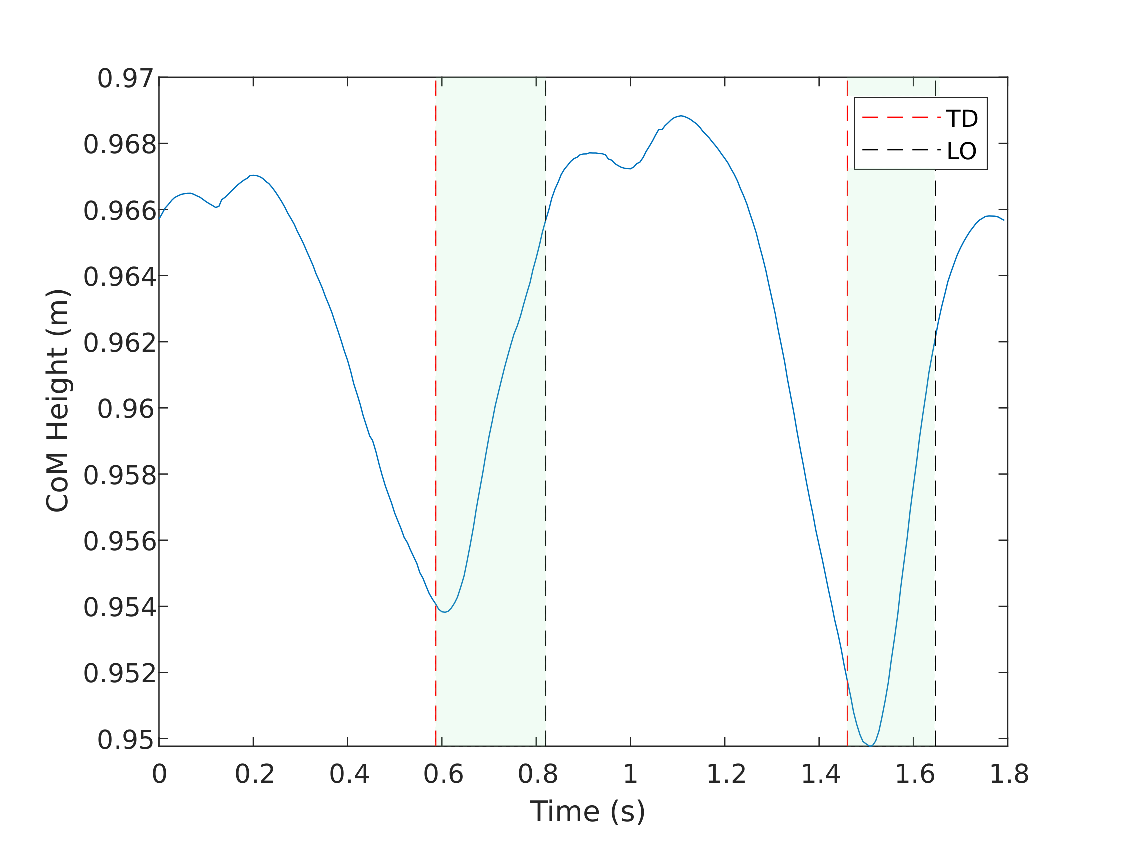
\includegraphics[width=\linewidth]{experimentalCoM.eps}}%
	\hfill
	\subcaptionbox{Vertical excursion of the \com~ of a 2D B-SLIP gait \label{fig:model_traj}}[0.49\textwidth]{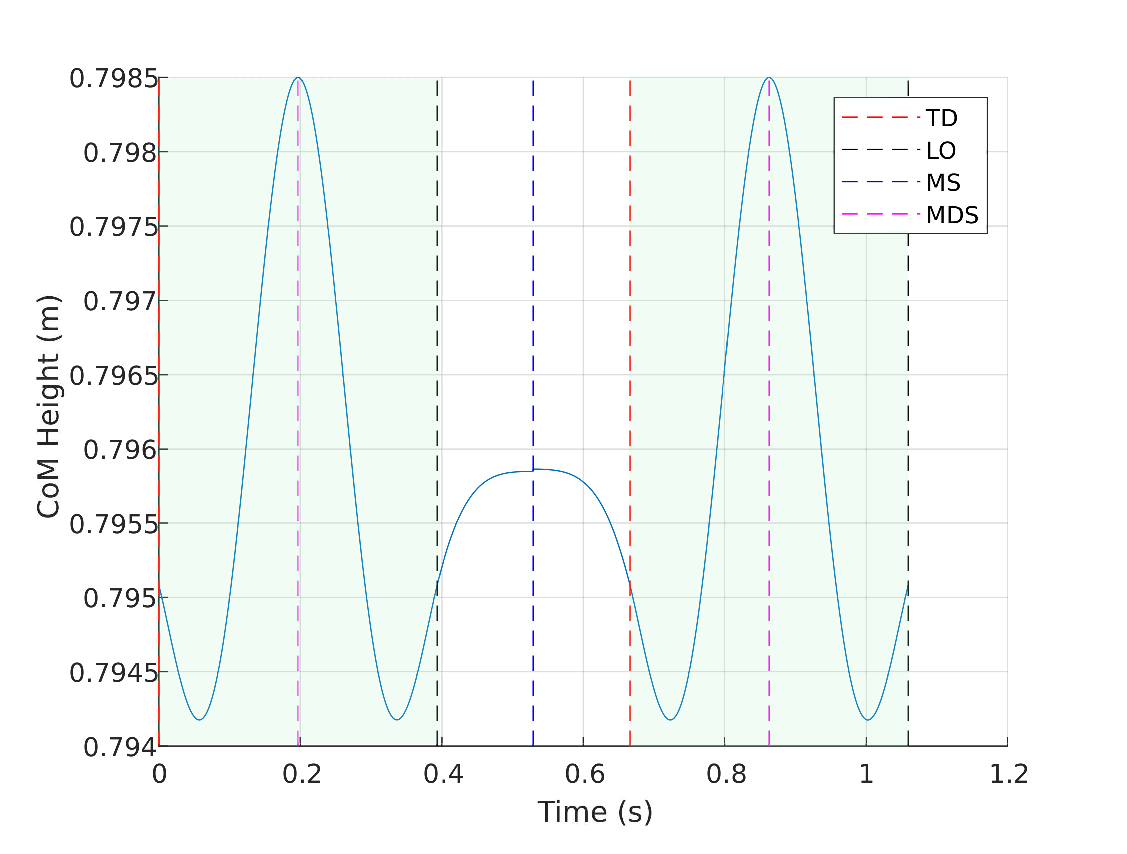
\includegraphics[width=\linewidth]{dSLIP.eps}}%
	\caption{Oscillations during the double-support (shaded green) of 2D B-SLIP gaits at low velocity} \label{fig:traj_compare}
\end{figure}

In their basic forms, the IP, SLIP, and B-SLIP models all ignore lateral dynamics, however, lateral dynamics become more dominant for low-speed gaits. For example, according to the human walking data presented by Fukuchi et al.~\cite{fukuchi2018public}, the peak-to-peak amplitude of the lateral sway of the CoM is approximately 3 cm while walking at 1.27 m/s but it rises to 9 cm while walking at 0.44 m/s. The model presented by Geyer is defined in only two dimensions, but it generalizes to 3D~\cite{liu2015dynamic,liu2016terrain}. This 3D model allows the lateral sway to be taken into consideration and oscillations during double support are eliminated. With appropriate leg length and step width, the sway seen in the gaits generated using the 3D B-SLIP model is comparable to human data. Considering the lateral sway is especially important while studying walking at low speeds. 

\subsection{Actuated Models}

Another approach to gait modeling is including a control input to achieve the desired gait. An example of this approach is the Variable-SLIP (V-SLIP) model, which uses variable stiffness actuation to modulate leg stiffness, in contrast to the original B-SLIP model, which has constant leg stiffness~\cite{visser2017bipedal}. This model produces a gait that is robust to disturbances, and whose cost of transport is comparable to human walking\footnote{Cost of transport quantifies the energy efficiency of a system, it measures the energy expended to travel a specified distance.}. Another approach is the Variable-Height Inverted Pendulum model, in which the CoM height is changed by applying a force along the leg~\cite{koolen2016balance} instead of varying leg stiffness. While all the previously described models have nonlinear dynamics, Kajita et al.~\cite{kajita1991study} proposed a model called the Linear Inverted Pendulum (LIP) model in which the application of a constrained control input linearizes the dynamics of the system where the height of the \com~ is specified. The LIP model also allows the use of ankle torques to improve model performance on rugged terrain. The LIP model has been extended to three dimensions with the 3D-LIP model~\cite{kajita20013d}.

Actuated models provide a more flexible framework to estimate gait, but determining the control parameters when applying those models to humans becomes a challenge. Therefore, active models are more suited to prosthetic devices which are used in series with the user or legged robots. Most active models have been proposed in regards to legged robots where the dynamics of the robot are well known to the designers. This allows for the complexity of the model to be matched to the complexity of the system dynamics. In the case of exoskeletons, the dynamics of the human body and a human's internal control system \cite{wolpert1998internal, dounskaia2005internal, kording2007decision} are still a subject of study and they are further complicated by the parallel operation with the exoskeleton suit due to coupling in the human and robot. The simplicity of passive models and the lack of a need to make assumptions about the inputs from a user working in parallel makes them more suited for parallel robots such as exoskeletons. As a result, passive models may be better suited for use in intent detection frameworks. 

\section{The B-SLIP model}\label{sec:bslip_model}
The work presented herein is focused on individuals recovering from iSCIs whose walking velocities were as low as 0.5 m/s. A majority of the duration of steps at low velocities is spent in double support, and it is important to use a model that can describe this gait phase. Therefore, this work considers a passive model, the 3D B-SLIP model, to model human locomotion shown in Fig~\ref{fig:slip}. In this model, the \COM~is loaded onto two massless spring legs of length $ l_o $ and stiffness $ k $. The state vector $ \x_{c} $ contains the position and velocity of the CoM, modeled by the point mass $ m $, relative to the stance foot such that $ \x_{c} = [x_{c} ,y_{c} ,z_{c} ,\dot{x}_{c} ,\dot{y}_{c} ,\dot{z}_{c}]^T $. The position of the leading leg at touchdown is given by two angles, the angle between the leading leg and vertical $ \theta $ and the angle $ \varphi $ between the forward axis $ x $  and the ground projection of the leading leg.
%
\begin{figure}
	\centering
	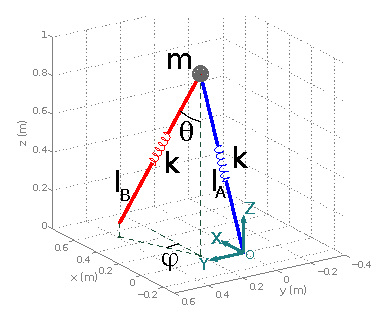
\includegraphics[width=0.5\linewidth]{3DSLIP.eps}
	\caption[The Bipedal Spring Loaded Inverted Pendulum]{The Bipedal Spring Loaded Inverted Pendulum \cite{liu2015dynamic} model of walking}\label{fig:slip}
\end{figure}
%
\begin{figure}
	\centering
	\includegraphics[width=0.85\linewidth]{slip_gait.pdf}
	\caption{One step of a B-SLIP gait}\label{fig:slip_gait}
\end{figure} 
%

A gait of the B-SLIP model, as viewed in the sagittal plane \footnote{The sagittal plane is the plane that divides the body into right and left parts.}, is illustrated in Fig.~\ref{fig:slip_gait}. This gait starts at midstance (MS), where the CoM is loaded onto the trailing leg in single-support (SS1). The gait then proceeds with the touchdown (TD) of the leading leg and enters the double support (DS) phase. The DS phase ends with lift-off (LO) of the trailing leg and the model enters the second single-support phase (SS2). The SS2 phase ends in MS, again with the CoM loaded onto the leading leg. As there are alternating SS and DS phases, the dynamics of the B-SLIP model are hybrid.

\subsection{Hybrid dynamics of the B-SLIP model}
The dynamics of the model in single support are described by
\begin{equation}
	m\ddot{\p}_{c} = k(l_0 - \lVert \mathbf{l}_i \rVert)\hat{\mathbf{l}}_i + m \mathbf{g}
\end{equation}
\noindent where $ i = \{A,B\} $ denotes the supporting leg, $ \mathbf{l}_i \in \mathbb{R}^3 $ is the vector along the leg from the mass to the position of the stance foot $\p_i$ , $ \hat{\mathbf{l}}_i \in \mathbb{R}^3$ is a unit vector along the leg, and $ \mathbf{g} \in \mathbb{R}^3 $ is the gravity vector. The dynamics during double support are given by
\begin{equation}
	m\ddot{\p}_{c} = k(l_0 - \lVert \mathbf{l}_A \rVert)\hat{\mathbf{l}}_A + k(l_0 - \lVert \mathbf{l}_B \rVert)\hat{\mathbf{l}}_B + m \mathbf{g}
\end{equation}
%
\noindent Certain conditions, known as guards, must be met to enable the switching of the dynamics from one phase to another. There are three switching surfaces to enable phase switches at TD, LO, and MS. These sets are as follows
%
\begin{eqnarray}
	\mathcal{G}_{TD} &=& \{(\p_c,\v_c)| \dot{z}_c < 0 ,z_{c} = z_{T}\} \label{eq:gtd} \\
	\mathcal{G}_{LO} &=& \{(\p_c,\v_c)| \dot{z}_c > 0 ,\lVert \mathbf{l}_A \rVert = l_0\} \label{eq:glo} \\
	\mathcal{G}_{MS} &=& \{(\p_c,\v_c)| \dot{z}_c = 0 ,z_{c} > z_{T} ,\lVert \mathbf{l}_A \rVert < l_0\} \label{eq:gms} 
\end{eqnarray} 
%
\noindent where $ z_{T} = l_0 \cos \theta $ is the threshold height for touchdown. Satisfaction of these guard conditions triggers gait phase switches and the states of the model are transferred across the switching events using functions called reset maps. For clarity of notation, let $ \z \in \mathbb{R}^{12} $ be the extended state that contains the CoM state and the positions of the feet such that
\[
	\z = \begin{bmatrix}
			\x_{c} \\
			\p_{A} \\
			\p_{B}
	\end{bmatrix}
\]
There are three reset maps following the general form $ \z^+ = h(\z^-,\u) $, where the $ + $ and $ - $ denote pre- and post-switch states. The first map is applied at TD when the guard \eqref{eq:gtd} is satisfied. There are no impacts at touchdown as spring legs of the B-SLIP model are assumed to be massless so the CoM state remains unchanged, and the position of the leading foot is updated as follows 
%\begin{gather}
%	\mathcal{R}_{TD}:\mathbb{R}^6 \rightarrow \mathbb{R}^6 \nonumber \\ 
%	\mathcal{R}_{TD}(\x^-) = \x^- 
%\end{gather}
\begin{eqnarray}
	\z^+ &=& h_{TD}(\z^-,\u) \qquad h_{TD}:\mathbb{R}^{12}\times \mathbb{R}^{3 \rightarrow } \mathbb{R}^{12} \\
	{}	&=& \begin{bmatrix}
		\x_{c}^- \\
		\p_{A}^- \\
		h_{TD}^{B}(\p_{c}^-, \u)
	\end{bmatrix} \nonumber
\end{eqnarray}
where
\begin{equation}
	h_{TD}^{B}(\p_{c}^-, \u) = \p_{c}^- + l_0%
	\begin{bmatrix}
		\sin(\theta)\cos(\phi)\\
		\sin(\theta)\sin(\phi)\\
		-\cos(\phi)
	\end{bmatrix}
\end{equation}
Were the feet assumed to have mass, this reset map would handle the impact event. The second map is applied as follows when the LO guard \eqref{eq:glo} is satisfied
%\begin{gather}
%	\mathcal{R}_{LO}:\mathbb{R}^6 \rightarrow \mathbb{R}^6 \nonumber \\ 
%	\mathcal{R}_{LO}(\x^-) = \x^- \\
%	\p_B \leftarrow \p_A \nonumber
%\end{gather}
\begin{eqnarray}
	\z^+ &=& h_{LO}(\z^-,\u) \qquad h_{LO}:\mathbb{R}^{12} \times \mathbb{R}^{3} \rightarrow \mathbb{R}^{12} \\
	{}	&=& \begin{bmatrix}
		\x_{c}^- \\
		\p_{B}^- \\
		\p_{B}^-
	\end{bmatrix} \nonumber
\end{eqnarray}
The model uses single-support dynamics after liftoff, so the labels of the foot are switched as the leg that was previously in swing will now be in stance, and the states remain unchanged. The last reset map is applied at MS when the guard \eqref{eq:gms} is met.
%
\begin{eqnarray}
	\z^+ &=& h_{MS}(\z^-,\u) \qquad h_{MS}:\mathbb{R}^{12}\times \rightarrow \mathbb{R}^{3} \mathbb{R}^{12} \\
	{}	&=& \begin{bmatrix}
		\D\x_{c}^- \\
		\p_{A}^- \\
		\p_{B}^-
	\end{bmatrix} \nonumber
\end{eqnarray}
%
%\begin{equation}
%	\mathcal{R}_{MS}:\x^- \rightarrowtail \p_{CoM} \leftarrow \x_{CoM} - \x_A :\mathbb{R}^6 \rightarrowtail \mathbb{R}^6
%\end{equation}
%
where $ \D = {\rm diag}([1 ,-1 ,1 ,1 ,-1 ,1 ,1]) $ to flip the signs of the lateral position and velocity of the CoM, as the state of the CoM is measured relative to the stance foot. Thus, the B-SLIP model can exhibit periodic gaits by alternately switching through SS and DS phases.

As the B-SLIP model is passive, it does not have any active control inputs to modify gaits and maintain periodicity. Therefore, optimization methods can be used to find periodic model gaits \cite{strogatz2018nonlinear,garcia1998simplest} as steady-state human walking is periodic. 

\section{Poincar\'e maps}

\begin{figure}
	\centering
	\includegraphics[width=.3\linewidth]{poincare.pdf}
	\caption{A Poincar\'e map used to find periodic gaits}\label{fig:poincare}
\end{figure}

Poincar\'e maps are used to study state flows near periodic orbits \cite{strogatz2018nonlinear}. Consider a system whose dynamics are $ \dot{\x} = f(\x) $ where $ \x \in \mathbb{R}^n $. Then a  Poincar\'e section for this system is a set with dimension of $ n-1 $ such that all trajectories passing through the section are transverse to it. It may be placed at a gait event such as MS, TD, or LO when the value of one of the states may be known, i.e., when a guard condition is met. Let the Poincar\'e section be placed at MS, let $ \x_k $ be the state at the $ k^{th} $ crossing of the section, and let $ \mathcal{P}(\x_k) $ be a function that returns the state after one cycle, or a step in the case of the B-SLIP, such that $ \x_{k+1} = \mathcal{P}(\x_k) $. The function $ \mathcal{P}(\x_k) $ is the Poincar\'e map formed by following trajectories from one intersection with the Poincar\'e section to the next, i.e., the Poincar\'e map takes a state on the Poincar\'e section and maps it back onto the section. There may exist an initial state, called a fixed point, representing a periodic orbit where the initial state maps back to itself after one period such that $ \x_k = \mathcal{P}(\x_k) $. 

Studying the behavior of the Poincar\'e maps simplifies a problem about periodic orbits to a problem about the fixed points of a map. Finding analytical solutions for $ \mathcal{P}(\x_k) $ may be difficult so numerical methods are often used. A Poincar\'e section placed at MS is shown in blue in Fig.~\ref{fig:poincare}. The dynamics of the model are integrated for one step using $ \x_k $ as the initial condition. Optimization methods are used to find initial conditions that yield periodic gait by minimizing the norm of $ \delta \x $, the error between $ \x_k $ and $ \x_{k+1} $. The nonlinear return map may be linearized about these periodic gaits for further refining the gait search as described in Chapter~\ref{chapter:IMM}. Model gaits for various velocities may be used as references while estimating an exoskeleton user's desired gait by comparing them with measurements of quantities such as \COM~height and velocity using state estimation tools such as the Kalman filter. 

\section{State estimation using Kalman filters}

Kalman filtering is a feedback-based sequential optimal estimation technique \cite{kalman1960new} to estimate states and parameters of dynamical systems. The estimates made by a Kalman filter are conditioned on certain measurements of either the states themselves or other quantities that may be represented as functions of the states through a measurement model. State estimation is reliant on these measurements to get a picture of the real world, however these measurements are rarely free of noise that may adversely affect the quality of the estimates. 

Kalman filters follow a predictor-corrector scheme in which states are propagated using a model of system dynamics which may be incomplete, and stochastic. These states are then corrected using the residual between sensor measurements and the predictions. If the feedback gain applied to this residual is too low, state estimates will not be appropriately corrected, and if the gain is too high, sensor noise will overshadow the system dynamics, and the estimates will begin tracking noise. Kalman filtering presents an optimal method of computing feedback gains that account for modeling and measurement errors with a fundamental assumption that any modeling or measurement errors are zero-mean Gaussian noise processes. The filter was originally proposed for discrete-time linear systems \cite{kalman1960new}. 
 
\subsection{Discrete-time Kalman Filter}
The filter is initialized at a certain initial state estimate $ \xh_0 $ that may have associated uncertainty due to measurement errors. The evolution of this state is described using dynamical system 
%
\begin{eqnarray}
	\x_{k+1} &=& \A_k \x_k + \B_k \u_k + \mathbf{G} \mathbf{w}_k,\quad \mathbf{w}_k \sim \mathcal{N}(0, \Q_k) \label{eq:sys_disc}  \\
	\yt_k &=& \H_k \x_k + \mathbf{v}_k,\quad \mathbf{v}_k \sim \mathcal{N}(0,\R_k) \label{eq:meas_lin}
\end{eqnarray}
%
\noindent where $ \x_k $ and $ \u_k $ are the discrete-time states and inputs, $ \y_k $ are the discrete-time measurements, $ \A_k $, $ \B_k $, $ \H_k $ are the system, input, and measurement models, respectively. The system is assumed to have zero-mean Gaussian noises for process noise $ \mathbf{w}_k $ and measurement noise $ \mathbf{v}_k $ with covariances  $ \Q_k $ and $ \R_k $, respectively. The measurement noise $ \mathbf{v}_k $ is combined with the measurement equation $ \H_k \x_k$ to form the noisy measurement $ \yt_k $. 
%
\begin{figure}
	\centering
	\includegraphics[width=0.7\linewidth]{kalman.pdf}
	\caption{Illustration of the Kalman Filtering process}\label{fig:kalman}
\end{figure}
%
The uncertainty associated with the estimates increases as the state is propagated forward through time using the system dynamics. Regular measurements of state variables are used to update the state estimates and reduce the uncertainty as illustrated in Fig.~\ref{fig:kalman} where the $ + $ and $ - $ in the superscript denote pre- and post-update states. The system illustrated here is discrete, however, a continuous state evolution is shown to better illustrate the growth in uncertainty. Kalman filters account for both the uncertainty in the state estimates and the measurements. Further details of this process are as follow. The state estimates and estimate covariance $ \P $ are propagated in discrete time such that
\begin{eqnarray}
	\xh_{k+1} &=& \A_k \xh_k + \B_k \u_k \\
	\P_{k+1} &=& \A_k\P_k \A_k^T + \mathbf{G}_k\Q_k\mathbf{G}_k^T 
\end{eqnarray}
\noindent The states are sequentially updated such that
\begin{eqnarray}
	\K_k &=& \P_k^- \H^T_k \left[\H_k \P_k^- \H^T_k + \R_k\right]^{-1} \label{eq:kalmanGain} \\
	\xh_k^+ &=& \xh_k^- + \K_k[\yt_k- \H_k \xh_k^-)] \label{eq:ekfStateUp} \\
	\P_k^+ &=& [\mathbf{I} - \K_k \H_k]\P_k^-\label{eq:ekfCovUp}
\end{eqnarray}
%
\noindent where the updated estimates, their covariance and the Kalman gain are $ \mathbf{x}_k^+ $, $ \mathbf{P}_k^+ $, and $ \K_k $, respectively. The Kalman gain is optimal and the error dynamics of the filter are shown to be stable \cite{Crassidis} using the Lyapunov candidate function $ V_k(\e_k) = \e_k^T \P_k^{-1} \e_k $ where $ \e_k \equiv \xh_k - \x_k $. The filter as described above is defined for linear systems, and it has been extended to nonlinear systems.

\subsection{Extended Kalman Filter}
Simple models used to describe legged locomotion have nonlinear dynamics, and so a variation of the Kalman filter named the Extended Kalman Filter (EKF) can be used for these systems. The nonlinear dynamics are linearized about the state estimate to work around the nonlinearity. As this linearization is an approximation of the dynamics, the EKF is not optimal like the discrete-time Kalman filter described previously. Despite the lack of optimality, EKFs have been in widespread use for nonlinear systems \cite{Crassidis, auger2013industrial}. Since most nonlinear dynamics are given in continuous time, a variation of the EKF called the Continuous-Discrete EKF may be used. In this variation, dynamics evolve in continuous time, and measurements are modeled in discrete time. This combination is used for estimation in the work presented herein as it most closely reflects the model and measurement conditions observed in the estimation problem being studied. The general structure of the EKF is similar to the filter presented previously, except the equations are nonlinear as seen by comparing \eqref{eq:sys_disc} and \eqref{eq:sys}. Consider the following nonlinear dynamical system
% Continuous-Discrete EKF
%
\begin{eqnarray}
	\dot{\x}(t) &=& \mathbf{f}(\x(t),\u(t),\mathbf{w}(t),t),\quad \mathbf{w}(t) \sim \mathcal{N}(0, \Q(t))  \label{eq:sys}  \\
	\yt_k &=& \mathbf{h}(\x_k) + \mathbf{v}_k,\quad \mathbf{v}_k \sim \mathcal{N}(0,\R_k) \label{eq:meas}
\end{eqnarray}
%
\noindent where $ \x(t) $ and $ \u(t) $ are the continuous-time states and inputs, $ \y_k $ are the discrete-time measurements, and $ \mathbf{f}(\x(t),\u(t),t) $ and $ \mathbf{h}(\x_k) $ are the system and measurement function respectively. The system has zero-mean Gaussian process and measurement noises $ \mathbf{w}(t) $ and $ \mathbf{v}_k $ respectively with covariances $ \Q(t) $ and $ \R_k $ respectively. The measurement noise $ \mathbf{v}_k $ is combined with the measurement equation $ \mathbf{h}(\x_k) $ to form the noisy measurement $ \yt_k $. 

The state estimates and estimate covariance $ \P $ are propagated in continuous time such that
\begin{eqnarray}
	\dot{\xh} &=& \mathbf{f}(\xh,\u,t) \label{eq:sysProp}\\
	\dot{\P}(t) &=& \F(t)\P(t) + \P(t)\F^T(t) + \mathbf{G}(t)\Q(t)\mathbf{G}(t)^T \label{eq:covProp} \\ 
	\F(t) &\equiv& \frac{\partial \mathbf{f}}{\partial \x} \Bigr |_{\xh(t),\u(t)} \nonumber
\end{eqnarray}
%
\noindent The states are sequentially updated such that
\begin{eqnarray}
	\K_k &=& \P_k^- \H^T_k(\xh_k^-) \left[\H_k(\xh_k^-)\P_k^- \H^T_k(\xh_k^-) + \R_k\right]^{-1} \\
	\xh_k^+ &=& \xh_k^- + \K_k[\yt_k-\mathbf{h}(\x_k)] \label{eq:sysUp} \\
	\P_k^+ &=& [\mathbf{I} - \K_k \H_k(\xh_k^-)]\P_k^-,\quad \H_k(\xh_k^-) \equiv \frac{\partial \mathbf{h}}{\partial \x} \Bigr |_{\xh_k^-}
\end{eqnarray}
%
\noindent where $ \K_k $ is the Kalman gain, $ \F(t) $, and $ \H_k(\xh_k^-) $ are the linearized dynamics and measurement model respectively. The updated estimates and their covariance are $ \mathbf{x}_k^+ $ and $ \mathbf{P}_k^+ $ respectively. The above equations describe a Continous-Discrete Kalman filter setup \cite{Crassidis}. System dynamics are propagated in continuous time \eqref{eq:sysProp} but states are updated in discrete time \eqref{eq:sysUp} since measurements are discrete. This setup handles the nonlinear dynamics of the models used to emulate legged locomotion however, it does not handle the hybrid nature of these models.

Each step of human walking has alternating single and double support periods depending on how many legs are in contact with the ground. Therefore, in addition to being nonlinear, models of legged locomotion have hybrid dynamics to describe different gait phases, i.e., different dynamics for different phases. The EKF can be used as an estimation tool to handle these hybrid dynamics in a framework known as Interacting Multi-Model (IMM) estimation. This framework allows the use of multiple EKFs in parallel and is discussed in detail in Chapter~\ref{chapter:IMM}.

\section{Exoskeleton data used for testing} \label{sec:exoData}
The estimation schemes presented in this work were all tested on walking trial data of users walking in an EksoGT exoskeleton (Fig.~\ref{fig:exoOperator})
developed by Ekso Bionics. The reliance of many state-of-the-art intent inference approaches on external sensors like electromyography (EMG) may be problematic in practical applications, as EMG sensors need consistency in placement and may slip during usage due to perspiration \cite{tkach2010study,ison2014role}. Therefore, this work strives to exclusively use measurements from sensors onboard the exoskeleton, as they may offer a more reliable option \cite{Gambon20b}, in addition to being cost-effective. 

\begin{figure}
	\centering
	\includegraphics[height=4in]{exo_gt.pdf}
	\vspace{-1em}
	\caption[Measurements obtained from sensors onboard the Ekso GT]{Measurements obtained from sensors onboard the Ekso GT \cite{eksoOperator}}\label{fig:exoOperator}
	\vspace{-1em}
\end{figure}

Trial data was collected as part of a study approved by the IRB of the University of Notre Dame (Protocol 18-04-4650) \cite{gambon2020effects}. The exoskeleton has two modes of operation, free and adaptive. Free mode is similar to gravity compensation whereas, in adaptive mode, the exoskeleton follows a predefined trajectory and corrects any deviations from it. This work uses data from trials of three uninjured and two injured users. Uninjured users underwent trials in both modes and injured users only underwent trials in adaptive mode. One of the injured users, IU-1, had a complete SCI at the middle of the spine (T5) and the second user, IU-2, had an incomplete SCI from the middle to the lower spine (T8 to L2). All users were highly experienced in the use of the EksoGT. The subjects used the exoskeleton at a self-selected speed with the assistance of a walker and were at a steady-state gait before being issued a verbal command to either speed up or slow down. The trial sequence was pseudo-random and each subject underwent three speed-up (SU) and slow-down (SD) trials for a total of six trials.

Sensors onboard the exoskeleton provide hip pitch, knee pitch, and torso pitch and roll angles, and are fused to estimate the height and fore-aft position of the hip in a global frame. These readings were used to approximate the location of the subject's CoM with respect to the stance foot. Since the position of the CoM is considered relative to the stance foot, the drift that may be present in the global position estimate does not affect step-to-step calculations. The subject's height, thigh, and shank lengths were recorded and the location of their CoM was approximated to be at the centroid of the pelvis. The remaining dimensions such as ankle height and hip-width were computed using anthropometry relationships defined by Winter \cite{winter2009biomechanics}. The CoM velocities and angular velocities of the joints and torso were computed with finite-difference approximations. Gait events identified for the estimator were MS, TD, and LO. A zero-crossing event between the left and right hip angles reported by the exoskeleton was used to detect MS. TD was detected when force sensor readings from both feet were above a threshold of 5\% of the maximum sensor value and LO was detected when the reading from the trailing foot fell below this threshold. 

\section{Summary}
This chapter serves as a repository of background information to help focus the subsequent chapters on their corresponding contributions. Poincar\'e maps were used during the generation a library containing gaits of the B-SLIP model. This library is used in the IMM framework for gait phase and velocity estimation as described in Chapter~\ref{chapter:IMM}. Kalman filters along with a Bayesian update stage form the basis of the estimators used in Chapters~\ref{chapter:BKF}~and~\ref{chapter:MP}. The IMM framework was tested synthetic data from simulated library gait and on the exoskeleton trial data described in Section \ref{sec:exoData}. The estimators used in Chapters~\ref{chapter:BKF}~and~\ref{chapter:MP} were tested solely on exoskeleton data.

	%
	% IMM
	\chapter{Model-based Approach to Estimate Gait Characteristics} \label{chapter:IMM}
	%
	% BKF
	\chapter{Intent Change Estimation Based on Physical Interactions of an	Exoskeleton User}\label{chapter:BKF}
	%
	% Model Personalization
	\chapter{Personalization of Estimation in the Presence of Data Scarcity}\label{chapter:MP}
	
	
	\appendix
	
	% If you have appendices, add them here.
	% Begin each one with \chapter{TITLE} as before. The \appendix command takes
	% care of renaming chapter headings and creates a new page in the Table of
	% Contents for them.
	% \include{appendix-one}
	
	\backmatter              % Place for bibliography and index
	
	
	\bibliographystyle{nddiss2e}
	\bibliography{references.bib}           % input the bib-database file name
	
	
\end{document}

%%
\endinput
%%
%% End of file `template.tex'.
